\documentclass[12pt,a4paper]{article}
\usepackage[utf8]{inputenc}
\usepackage[margin=1in]{geometry}
\usepackage{graphicx}
\usepackage{amsmath}
\usepackage{amsfonts}
\usepackage{enumerate}
\usepackage{listings}
\usepackage{xcolor}
\usepackage{float}
\usepackage{booktabs}

\definecolor{codegreen}{rgb}{0,0.6,0}
\definecolor{codegray}{rgb}{0.5,0.5,0.5}
\definecolor{codepurple}{rgb}{0.58,0,0.82}
\definecolor{backcolour}{rgb}{0.95,0.95,0.92}

\lstdefinestyle{mystyle}{
    backgroundcolor=\color{backcolour},   
    commentstyle=\color{codegreen},
    keywordstyle=\color{blue},
    numberstyle=\tiny\color{codegray},
    stringstyle=\color{codepurple},
    basicstyle=\sffamily\footnotesize,
    breakatwhitespace=false,         
    breaklines=true,                 
    captionpos=b,                    
    keepspaces=true,                 
    numbers=left,                    
    numbersep=5pt,                  
    showspaces=false,                
    showstringspaces=false,
    showtabs=false,                  
    tabsize=4
}

\lstset{style=mystyle}

% Title and Author
\title{TMA4162 Computational algebra, Project 2}
\author{Andreas Moe}
\date{\today}

\begin{document}

\maketitle

\section*{Task 1, Theory}
Define \(S_n = \{2^n, 2^n+1, ... , 2^{n+1}-1\}\)
\begin{enumerate}[a)]
    \item 
    Let \(X\) be a uniform random variable over \(S_n\).
    \[
    Let\ p = P(X\ is\ a\ prime) = \frac{number\ of\ primes\ in\ S_n}{|s_n|}
    = \frac{\pi(2^{n+1}-1) - \pi(2^n-1)}{2^n} \]
    \[\approx 
    2^{-n}\left(\frac{2^{n+1}}{log(2^{n+1})}-\frac{2^n}{log(2^n)}\right)
    = \frac{2}{(n+1)\ log\ 2}-\frac{1}{n\ log\ 2}
    = \frac{2n - (n+1)}{(n+1)n\ log\ 2}
    \]
    \[
    \approx \frac{1}{n\ log 2}
    \]
    We are interested in the expected number of candidates that must be tested before a prime is found. The number of failed candidates follows a negative binomial distribution with one success (r=1). The expected number of trials to see \(r\) successes in a negative binomial distribution is \(\frac{r}{p} = \frac{1}{p}\) in our case.
    The expected number of trials is therefore \(\approx \mathbf{n\ log\ 2}\).

    \begin{table}[H]
        \begin{table}
\label{tab:exp_candidates}
\begin{tabular}{rr}
\toprule
n & Candidates \\
\midrule
10 & 6.931472 \\
50 & 34.657359 \\
100 & 69.314718 \\
500 & 346.573590 \\
1000 & 693.147181 \\
\bottomrule
\end{tabular}
\end{table}

    \end{table}

    \end{enumerate}

\section*{Task 2, Practice}

\begin{enumerate}[a)]
    \item 

\end{enumerate}

\begin{figure}[htbp]
    \centering
    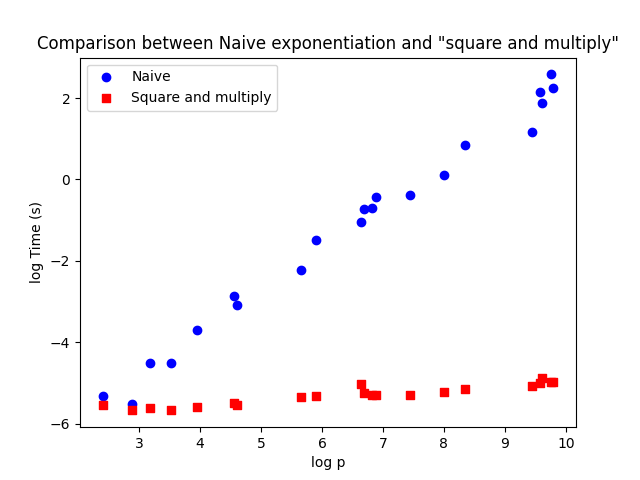
\includegraphics[width=\linewidth]{plot_2025-01-24 14-39-00_0.png}
    \caption{Measurements}
    \label{figure1}
\end{figure}
\newpage
\begin{appendix}
\section*{Appendix}
    Code is available at https://github.com/andrmoe/ComputationalAlgebra
    \lstinputlisting[language=Python, caption={prime.py}, label={lst:python_code1}]{prime.py}
    \lstinputlisting[language=Python, caption={test.py}, label={lst:python_code2}]{test.py}
\end{appendix}

\end{document}
